---
id: tkz-euclide-ejemplo-53
title: "Ángulo recto"
description: "Creación de un ángulo recto"
keywords: [angulo,recto,rayo,taller1]
tags: [tkzDefShiftPoint,tkzFillAngle,tkzMarkAngle,tkzDrawLines]
sort: 53
---
\documentclass[tikz,border=2mm]{standalone}
\usepackage{tkz-base}
\usepackage{tkz-euclide}

\begin{document}
    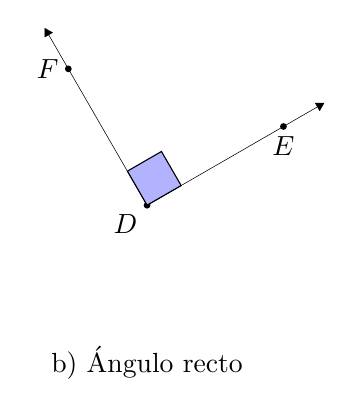
\begin{tikzpicture}                        
        % Paso 1: Define vértice del ángulo
        \tkzDefPoint(7,2){D}

        % Paso 2: Define punto del rayo inferior a 30° de D
        \tkzDefShiftPoint[D](30:2){E}
        % Paso 3: Define punto del rayo inferior a 120° de D
        \tkzDefShiftPoint[D](120:2){F}
        
        % Paso 4: Dibuja los puntos y etiquétalos
        \tkzDrawPoints(D,E,F)
        \tkzLabelPoints[below left](D)
        \tkzLabelPoints[below](E)
        \tkzLabelPoints[left](F)

        % Paso 5: Marca y rellena el ángulo
        \tkzMarkRightAngle[fill=blue!30,size=0.5](E,D,F) % ∠EDF

        % Paso 6: Dibuja los segmentos de los rayos
        \tkzDrawLines[add=0 and 0.3, -Triangle](D,F D,E)

        % Paso 7: Agrega leyenda al gráfico
        \tkzText(7,0){b) Ángulo recto}        
    \end{tikzpicture}
\end{document}
